\documentclass[12pt]{article}
% controlling the geometry of the page:
\usepackage[margin=1in, paperwidth=8.5in, paperheight=11in]{geometry} 
\usepackage{amsmath, amssymb} % useful math symbols and environments

\usepackage{multicol} % multiple columns side-by-side

\usepackage{amsthm} % Theorem-like environments
\theoremstyle{definition} % Without this line, theorem statements (and therefore problem statements etc.) show up in italic text.
\newtheorem{conjecture}{Conjecture}
\newtheorem{problem}{Problem}
\newtheorem*{remark}{Remark}
\newtheorem*{problem*}{Problem}
% pretty colors!
\usepackage[dvipsnames]{xcolor}
\colorlet{darkgrey}{black!70}
\colorlet{darkgreen}{green!50!black}


\usepackage{tikz} % for drawing diagrams
\usetikzlibrary{arrows,automata,positioning} 
\usetikzlibrary{decorations.markings}
\usetikzlibrary{decorations.pathreplacing}
\usetikzlibrary{patterns}
\usetikzlibrary{shapes.geometric}

%%---------------------------------------------------------------------------
%% included from visualalgebra.sty (see the beamer folder)
%% TEXT COLORS
%%
\definecolor{xRed}{rgb}{.9,0,0}       
\definecolor{xBlue}{rgb}{0,0,.9}      
\definecolor{xGreen}{HTML}{009000}   %% "Islamic green"
\definecolor{xPurple}{HTML}{D14FFF}  
\definecolor{xOrange}{HTML}{F56600}  %% "Clemson orange"

\newcommand{\Alert}[1]{\textcolor{xRed}{#1}}
\newcommand{\Balert}[1]{\textcolor{xBlue}{#1}}
\newcommand{\Galert}[1]{\textcolor{xGreen}{#1}}
\newcommand{\Palert}[1]{\textcolor{xPurple}{#1}}
\newcommand{\Oalert}[1]{\textcolor{xOrange}{#1}}
\newcommand{\Walert}[1]{\textcolor{white}{#1}}

%% vertices in cayley graphs
\tikzset{v/.style={circle, draw, fill=lightgray,inner sep=0pt, 
  minimum size=6mm}}

%% Edge colors
%%
\definecolor{eRed}{rgb}{1,0,0}      % Cayley diagram edges
\definecolor{eBlue}{rgb}{0,0,1}     % Cayley diagram edges
\definecolor{eGreen}{HTML}{7EC636}  % Goodnotes green (a little darker)
\definecolor{eGreen}{HTML}{3CAC13}  % I like this a litte better
\definecolor{ePurple}{HTML}{D287FF} % Close to goodnotes 
\colorlet{eOrange}{orange}

% Edge styles 
%%
\tikzset{r/.style={draw, very thick, eRed, -stealth}}  % Red -->
\tikzset{rr/.style={draw, very thick, eRed}}           % Red ---
\tikzset{r2/.style={draw, very thick, eRed,stealth'-stealth'}} % Red <-->
\tikzset{b/.style={draw, very thick, eBlue, -stealth}} % Blue -->
\tikzset{bb/.style={draw, very thick, eBlue}}          % Blue ---
\tikzset{b2/.style={draw, very thick, eBlue,stealth'-stealth'}} % Blue <-->
\tikzset{g/.style={draw, very thick, eGreen, -stealth}} % Green -->
\tikzset{gg/.style={draw, very thick, eGreen}}          % Green ---
\tikzset{g2/.style={draw, very thick, eGreen,stealth'-stealth'}} % Green <-->
\tikzset{p/.style={draw, very thick, ePurple, -stealth}} % Purple -->
\tikzset{pp/.style={draw, very thick, ePurple}}           % Purple ---
\tikzset{p2/.style={draw, very thick, ePurple,stealth'-stealth'}} % Purple <-->
\tikzset{o/.style={draw, very thick, eOrange, -stealth}} % Orange -->
\tikzset{oo/.style={draw, very thick, eOrange}}           % Orange ---
\tikzset{o2/.style={draw, very thick, eOrange,stealth'-stealth'}} % Orange <-->
%%
\tikzstyle{cy2} = [draw,very thick]           %% cycle graph edges
\definecolor{faded}{rgb}{.75,.75,.75}
\tikzstyle{f} = [faded]                         % This is used all the time
%%---------------------------------------------------------------------------
%%
%% COLORS FOR COSET BUBBBLES 
%%
\colorlet{cosetGray}{gray!15!white}
\colorlet{cosetBlue}{blue!15!white}
\colorlet{cosetRed}{red!15!white}
\definecolor{cosetPurple}{rgb}{.9 .84 .965}
\definecolor{cosetGreen}{rgb}{.863 .92 .855}
%%---------------------------------------------------------------------------

\usepackage{graphicx} % for inserting figures with \includegraphics
\usepackage{setspace} % for controlling space between lines, paragraphs, etc.

\usepackage{fancyhdr} % for controlling headers and footers
\usepackage{newtx} % changes the default font family
\usepackage[shortlabels]{enumitem} % controllable labels for ordered and unordered lists

\usepackage{hyperref} % controls hyperlinks, both internal and external
\hypersetup{
    colorlinks=true,
    urlcolor=blue,
}

\setlength{\headheight}{14.5pt}
\newcommand{\Q}{\mathbb{Q}}
\newcommand{\R}{\mathbb{R}}
\newcommand{\Z}{\mathbb{Z}}
\newcommand\inv{^{-1}} % I am very tired of typing ^{-1}
\def\<{\langle}
\def\>{\rangle}
\DeclareMathOperator\Rect{\mathbf{Rect}}
\DeclareMathOperator\Tri{\mathbf{Tri}}
\DeclareMathOperator\Sq{\mathbf{Sq}}
\DeclareMathOperator\Light{\mathbf{Light}}
\DeclareMathOperator{\lcm}{lcm}
%% Abstract algebra commands
\def\normal{\lhd}
\def\normaleq{\unlhd}
\def\nnormal{\ntriangleleft}
\def\nnormaleq{\ntrianglelefteq}

\newenvironment{red}{\color{red}}{\ignorespacesafterend}

% I don't like how LaTeX renders section headings by default
\renewcommand{\section}[1]{\begin{center} \textbf{#1} \\\end{center}}
%
\setlength{\parindent}{0in}
%\oddsidemargin=-.25in
\allowdisplaybreaks
\pagestyle{fancy}
\renewcommand{\headrulewidth}{0pt}
\lhead{MATH 312}
\rhead{Spring 2025}
%\lfoot{\copyright\ CLEAR Calculus 2010}
\cfoot{}
\renewcommand{\thefootnote}{*} 
\hyphenpenalty=10000 % LaTeX by default really likes hyphenating things

% all the stuff above this line is called the preamble...
%##################################################################
\begin{document} % this is always the first line of what's actually produced
\section{Problem 9 from Homework \#5} % notice that if you want the character # to appear, you have to "escape" it with a backslash

\begin{problem*}\label{A4-cosets}
    Here's an extended problem where you can explore the relationship between left cosets, right cosets, conjugate subgroups, and normalizers.

    Below are three Cayley diagrams of $A_4$, each highlighting the left cosets of a different subgroup. These are the subgroups $N$, $H$, and $K$ from slide 17 of the normal-subgroups slides from class on Wednesday. To make the notation suck less and the Cayley diagrams more readable, we can take $\Alert{a=(123)}$, $\Palert{b=(134)}$, $\Balert{x=(12)(34)}$, and $\Galert{z=(13)(24)}$; arrows in the Cayley diagrams are color-coded appropriately. Then:
    \[N = \<\Balert{x}, \Galert{z}\>; \qquad H = \<\Alert{a}\>; \qquad K = \<\Balert{x}\>.\]
    \vspace{-15mm}

    \[
    \hspace*{-3mm}
    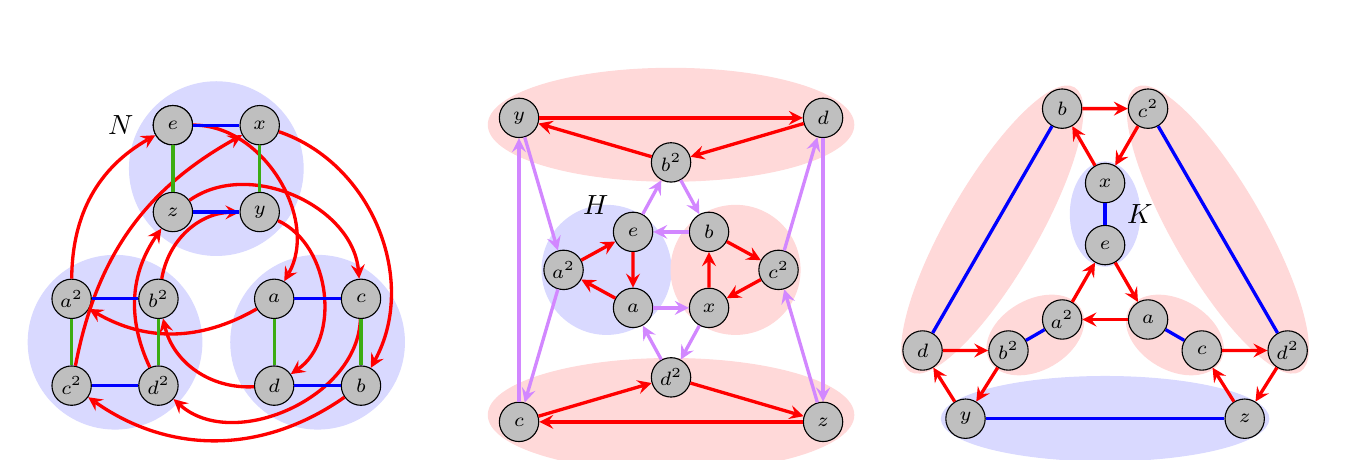
\begin{tikzpicture}[scale=1.05]
        \tikzstyle{v} = [circle, draw, fill=lightgray,inner sep=0pt,
        minimum size=5mm]
        \tikzstyle{every node}=[font=\scriptsize]
        %% N version
        \begin{scope}[shift={(0,-1.1)},scale=.7] 
            \draw[cosetBlue, fill=cosetBlue] (.75,.75) circle (15mm);
            \draw[cosetBlue, fill=cosetBlue] (4.25,.75) circle (15mm);
            \draw[cosetBlue, fill=cosetBlue] (2.5,3.75) circle (15mm);
            \node (e) at (1.75,4.5) [v] {$e$};
            \node (x) at (3.25,4.5) [v] {$x$};
            \node (z) at (1.75,3) [v] {$z$};
            \node (y) at (3.25,3) [v] {$y$};
            \node (a) at (3.5,1.5) [v] {$a$};
            \node (c) at (5,1.5) [v] {$c$};
            \node (d) at (3.5,0) [v] {$d$};
            \node (b) at (5,0) [v] {$b$};
            \node (dd) at (1.5,0) [v] {$d^2$};
            \node (bb) at (1.5,1.5) [v] {$b^2$};
            \node (aa) at (0,1.5) [v] {$a^2$};
            \node (cc) at (0,0) [v] {$c^2$};
            \draw [r] (x) to [bend left=50] (b);
            \draw [r] (e) to [bend left=60] (a);
            \draw [r] (z) to [bend left=60] (c);
            \draw [r] (y) to [bend left=60] (d);
            \draw [r] (a) to [bend left] (aa);
            \draw [r] (b) to [bend left=35] (cc);
            \draw [r] (c) to [bend left=65] (dd);
            \draw [r] (d) to [bend left=40] (bb);
            \draw [r] (aa) to [bend left] (e);
            \draw [r] (bb) to [bend left=40] (y);
            \draw [r] (cc) to [bend left=25] (x);
            \draw [r] (dd) to [bend left] (z);
            \node at (1.75,4.5) [v] {$e$};
            \node at (.85,4.5) {\normalsize$N$};
            \draw [bb] (e) to (x);
            \draw [bb] (z) to (y);
            \draw [gg] (e) to (z);
            \draw [gg] (x) to (y);
            \draw [bb] (a) to (c);
            \draw [bb] (d) to (b);
            \draw [gg] (a) to (d);
            \draw [gg] (c) to (b);
            \draw [bb] (aa) to (bb);
            \draw [bb] (cc) to (dd);
            \draw [gg] (aa) to (cc);
            \draw [gg] (bb) to (dd);
        \end{scope}
        %% K version
        \begin{scope}[shift={(12.5,0)},scale=.6]
            \draw[cosetBlue, fill=cosetBlue] (0,1.625) ellipse (.7 and 1.05);
            \draw[color=cosetRed,fill=cosetRed] (-1.407,-.8125)
            circle [x radius=.7cm, y radius=1.05cm, rotate=-60];
            \draw[color=cosetRed,fill=cosetRed] (1.407,-.8125)
            circle [x radius=.7cm, y radius=1.05cm, rotate=60];
            \draw[cosetBlue, fill=cosetBlue] (0,-2.5) ellipse (3.3 and .85);
            \draw[color=cosetRed,fill=cosetRed] (2.273,1.3125)
            circle [x radius=.9cm, y radius=3.3cm, rotate=30];
            \draw[color=cosetRed,fill=cosetRed] (-2.273,1.3125)
            circle [x radius=.9cm, y radius=3.3cm, rotate=-30];
            \node (l1) at (0,2.25) [v] {$x$};
            \node (l2) at (-.866,3.75) [v] {$b$};
            \node (t1) at (0,1) [v] {$e$};
            \node (t2) at (-.866,-.5) [v] {$a^2$};
            \node (t3) at (.866,-.5) [v] {$a$};
            \node (l3) at (.866,3.75) [v] {$c^2$};
            \node (r1) at (3.68,-1.125) [v] {$d^2$};
            \node (r2) at (2.814,-2.5) [v] {$z$};
            \node (r3) at (1.948,-1.125) [v] {$c$};
            \node (m2) at (-1.948,-1.125) [v] {$b^2$};
            \node (m1) at (-3.68,-1.125) [v] {$d$};
            \node (m3) at (-2.814,-2.5) [v] {$y$};
            \node at (.7,1.625) {\normalsize$K$};
            \draw [bb] (l2) to (m1);
            \draw [bb] (m2) to (t2);
            \draw [bb] (r2) to (m3);
            \draw [bb] (l1) to (t1);
            \draw [bb] (l3) to (r1);
            \draw [bb] (r3) to (t3);
            \draw [r] (l1) to (l2);
            \draw [r] (l2) to (l3);
            \draw [r] (l3) to (l1);
            \draw [r] (t1) to (t3);
            \draw [r] (t2) to (t1);
            \draw [r] (t3) to (t2);
            \draw [r] (r1) to (r2);
            \draw [r] (r2) to (r3);
            \draw [r] (r3) to (r1);
            \draw [r] (m1) to (m2);
            \draw [r] (m2) to (m3);
            \draw [r] (m3) to (m1);
        \end{scope}
        %% H version
        \begin{scope}[shift={(7.25,.3)},scale=.65]
            \draw[cosetBlue, fill=cosetBlue] (-1.2,0) circle (1.2);
            \draw[cosetRed, fill=cosetRed] (1.2,0) circle (1.2);
            \draw[cosetRed, fill=cosetRed] (0,2.7) ellipse (3.4 and 1.05);
            \draw[cosetRed, fill=cosetRed] (0,-2.7) ellipse (3.4 and 1.05);
            \node (a2) at (45:1) [v] {$b$};
            \node (a4) at (135:1) [v] {$e$}; %{$\tiny *$};
            \node (a6) at (225:1) [v] {$a$};
            \node (a8) at (315:1) [v] {$x$};
            \node (b1) at (0:2) [v] {$c^2$};
            \node (b3) at (90:2) [v] {$b^2$};
            \node (b5) at (180:2) [v] {$a^2$};
            \node (b7) at (270:2) [v] {$d^2$};
            \node (c2) at (45:4) [v] {$d$};
            \node (c4) at (135:4) [v] {$y$};
            \node (c6) at (225:4) [v] {$c$};
            \node (c8) at (315:4) [v] {$z$};
            \node at (-1.4,1.2) {\normalsize$H$};
            \draw [r] (b1) to (a8); \draw [r] (a8) to (a2); \draw [r] (a2) to (b1);
            \draw [r] (a4) to (a6); \draw [r] (a6) to (b5); \draw [r] (b5) to (a4);
            \draw [r] (c2) to (b3); \draw [r] (b3) to (c4); \draw [r] (c4) to (c2);
            \draw [r] (c6) to (b7); \draw [r] (b7) to (c8); \draw [r] (c8) to (c6);
            \draw [p] (b1) to (c2); \draw [p] (c2) to (c8); \draw [p] (c8) to (b1);
            \draw [p] (b5) to (c6); \draw [p] (c6) to (c4); \draw [p] (c4) to (b5);
            \draw [p] (b3) to (a2); \draw [p] (a2) to (a4); \draw [p] (a4) to (b3);
            \draw [p] (a6) to (a8); \draw [p] (a8) to (b7); \draw [p] (b7) to (a6);
        \end{scope}
    \end{tikzpicture}
    \]
    \begin{enumerate}[(a)]
        \item Label each of the ``coset bubbles'' in each diagram above with which left coset it is. For instance, $\{a, c, b, d\}$ is certainly $aN$.
        \item For each subgroup shown above, partition $A_4$ into its right
        cosets. (Work smarter not harder: think about which elements you actually need to bother shifting by!)
        Write the right cosets as subsets of $A_4$, consisting of permutations
        in cycle notation. Also, highlight them by colors on a fresh copy
        of the Cayley diagrams -- see the next page.
        \item Conjecture as to why I made some of the bubbles blue and some of them red. Relatedly, find $N_{A_4}(N)$, $N_{A_4}(H)$, and $N_{A_4}(K)$.
        \item For each (non-identity) left coset $gH$, illustrate the construction of the
        conjugate subgroup $gHg^{-1}$ on a fresh copy of the Cayley
        diagram -- see next page. Repeat this for $N$ and $K$. \\
    \end{enumerate}
\end{problem*}

%%======================================================================
\subsection*{Fresh Cayley diagrams for Problem \ref{A4-cosets}}

Please please \textit{please} print this out and draw your coset bubbles by hand (or by marking up a pdf on a tablet). I promise that it would suck \textit{so much} to do this in tikz.

\vspace{5mm}

For part (b):
\[
    \hspace*{-3mm}
    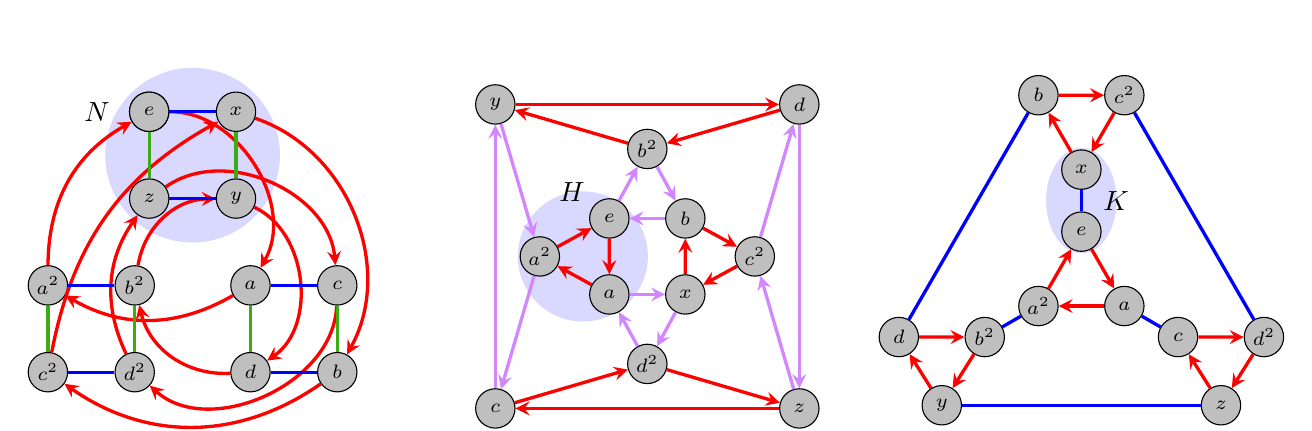
\begin{tikzpicture}[scale=1.05]
        \tikzstyle{v} = [circle, draw, fill=lightgray,inner sep=0pt,
        minimum size=5mm]
        \tikzstyle{every node}=[font=\scriptsize]
        %% N version
        \begin{scope}[shift={(0,-1.1)},scale=.7] 
            \draw[cosetBlue, fill=cosetBlue] (2.5,3.75) circle (15mm);
            \node (e) at (1.75,4.5) [v] {$e$};
            \node (x) at (3.25,4.5) [v] {$x$};
            \node (z) at (1.75,3) [v] {$z$};
            \node (y) at (3.25,3) [v] {$y$};
            \node (a) at (3.5,1.5) [v] {$a$};
            \node (c) at (5,1.5) [v] {$c$};
            \node (d) at (3.5,0) [v] {$d$};
            \node (b) at (5,0) [v] {$b$};
            \node (dd) at (1.5,0) [v] {$d^2$};
            \node (bb) at (1.5,1.5) [v] {$b^2$};
            \node (aa) at (0,1.5) [v] {$a^2$};
            \node (cc) at (0,0) [v] {$c^2$};
            \draw [r] (x) to [bend left=50] (b);
            \draw [r] (e) to [bend left=60] (a);
            \draw [r] (z) to [bend left=60] (c);
            \draw [r] (y) to [bend left=60] (d);
            \draw [r] (a) to [bend left] (aa);
            \draw [r] (b) to [bend left=35] (cc);
            \draw [r] (c) to [bend left=65] (dd);
            \draw [r] (d) to [bend left=40] (bb);
            \draw [r] (aa) to [bend left] (e);
            \draw [r] (bb) to [bend left=40] (y);
            \draw [r] (cc) to [bend left=25] (x);
            \draw [r] (dd) to [bend left] (z);
            \node at (1.75,4.5) [v] {$e$};
            \node at (.85,4.5) {\normalsize$N$};
            \draw [bb] (e) to (x);
            \draw [bb] (z) to (y);
            \draw [gg] (e) to (z);
            \draw [gg] (x) to (y);
            \draw [bb] (a) to (c);
            \draw [bb] (d) to (b);
            \draw [gg] (a) to (d);
            \draw [gg] (c) to (b);
            \draw [bb] (aa) to (bb);
            \draw [bb] (cc) to (dd);
            \draw [gg] (aa) to (cc);
            \draw [gg] (bb) to (dd);
        \end{scope}
        %% K version
        \begin{scope}[shift={(12.5,0)},scale=.6]
            \draw[cosetBlue, fill=cosetBlue] (0,1.625) ellipse (.7 and 1.05);
            \node (l1) at (0,2.25) [v] {$x$};
            \node (l2) at (-.866,3.75) [v] {$b$};
            \node (t1) at (0,1) [v] {$e$};
            \node (t2) at (-.866,-.5) [v] {$a^2$};
            \node (t3) at (.866,-.5) [v] {$a$};
            \node (l3) at (.866,3.75) [v] {$c^2$};
            \node (r1) at (3.68,-1.125) [v] {$d^2$};
            \node (r2) at (2.814,-2.5) [v] {$z$};
            \node (r3) at (1.948,-1.125) [v] {$c$};
            \node (m2) at (-1.948,-1.125) [v] {$b^2$};
            \node (m1) at (-3.68,-1.125) [v] {$d$};
            \node (m3) at (-2.814,-2.5) [v] {$y$};
            \node at (.7,1.625) {\normalsize$K$};
            \draw [bb] (l2) to (m1);
            \draw [bb] (m2) to (t2);
            \draw [bb] (r2) to (m3);
            \draw [bb] (l1) to (t1);
            \draw [bb] (l3) to (r1);
            \draw [bb] (r3) to (t3);
            \draw [r] (l1) to (l2);
            \draw [r] (l2) to (l3);
            \draw [r] (l3) to (l1);
            \draw [r] (t1) to (t3);
            \draw [r] (t2) to (t1);
            \draw [r] (t3) to (t2);
            \draw [r] (r1) to (r2);
            \draw [r] (r2) to (r3);
            \draw [r] (r3) to (r1);
            \draw [r] (m1) to (m2);
            \draw [r] (m2) to (m3);
            \draw [r] (m3) to (m1);
        \end{scope}
        %% H version
        \begin{scope}[shift={(7.25,.3)},scale=.65]
            \draw[cosetBlue, fill=cosetBlue] (-1.2,0) circle (1.2);
            \node (a2) at (45:1) [v] {$b$};
            \node (a4) at (135:1) [v] {$e$}; %{$\tiny *$};
            \node (a6) at (225:1) [v] {$a$};
            \node (a8) at (315:1) [v] {$x$};
            \node (b1) at (0:2) [v] {$c^2$};
            \node (b3) at (90:2) [v] {$b^2$};
            \node (b5) at (180:2) [v] {$a^2$};
            \node (b7) at (270:2) [v] {$d^2$};
            \node (c2) at (45:4) [v] {$d$};
            \node (c4) at (135:4) [v] {$y$};
            \node (c6) at (225:4) [v] {$c$};
            \node (c8) at (315:4) [v] {$z$};
            \node at (-1.4,1.2) {\normalsize$H$};
            \draw [r] (b1) to (a8); \draw [r] (a8) to (a2); \draw [r] (a2) to (b1);
            \draw [r] (a4) to (a6); \draw [r] (a6) to (b5); \draw [r] (b5) to (a4);
            \draw [r] (c2) to (b3); \draw [r] (b3) to (c4); \draw [r] (c4) to (c2);
            \draw [r] (c6) to (b7); \draw [r] (b7) to (c8); \draw [r] (c8) to (c6);
            \draw [p] (b1) to (c2); \draw [p] (c2) to (c8); \draw [p] (c8) to (b1);
            \draw [p] (b5) to (c6); \draw [p] (c6) to (c4); \draw [p] (c4) to (b5);
            \draw [p] (b3) to (a2); \draw [p] (a2) to (a4); \draw [p] (a4) to (b3);
            \draw [p] (a6) to (a8); \draw [p] (a8) to (b7); \draw [p] (b7) to (a6);
        \end{scope}
    \end{tikzpicture}
\]

For part (d), subgroup $H$ (3 copies bc $[A_4:H] = 4$ and I don't care about one of 'em):

\[
    \hspace*{-3mm}
    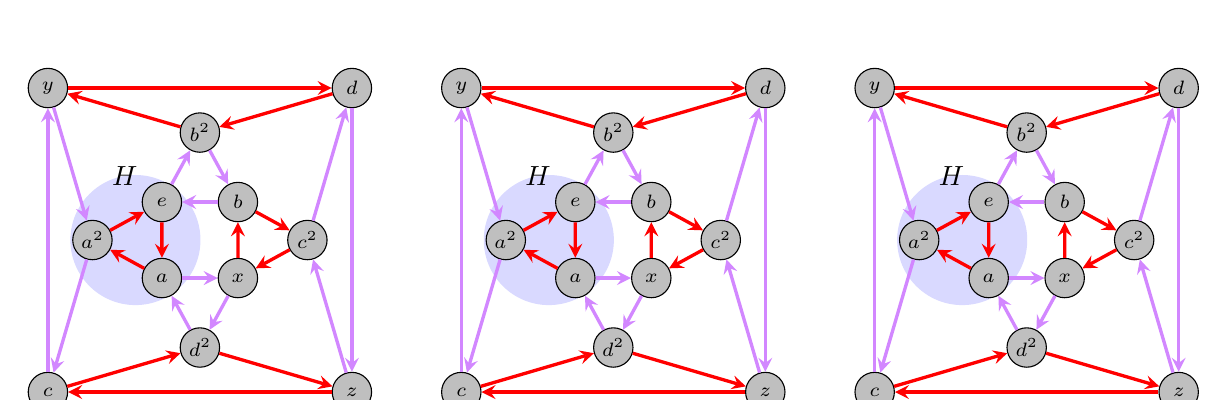
\begin{tikzpicture}[scale=1.05]
        \tikzstyle{v} = [circle, draw, fill=lightgray,inner sep=0pt,
        minimum size=5mm]
        \tikzstyle{every node}=[font=\scriptsize]
        %% H version
        \begin{scope}[shift={(0,.3)},scale=.65]
            \draw[cosetBlue, fill=cosetBlue] (-1.2,0) circle (1.2);
            \node (a2) at (45:1) [v] {$b$};
            \node (a4) at (135:1) [v] {$e$}; %{$\tiny *$};
            \node (a6) at (225:1) [v] {$a$};
            \node (a8) at (315:1) [v] {$x$};
            \node (b1) at (0:2) [v] {$c^2$};
            \node (b3) at (90:2) [v] {$b^2$};
            \node (b5) at (180:2) [v] {$a^2$};
            \node (b7) at (270:2) [v] {$d^2$};
            \node (c2) at (45:4) [v] {$d$};
            \node (c4) at (135:4) [v] {$y$};
            \node (c6) at (225:4) [v] {$c$};
            \node (c8) at (315:4) [v] {$z$};
            \node at (-1.4,1.2) {\normalsize$H$};
            \draw [r] (b1) to (a8); \draw [r] (a8) to (a2); \draw [r] (a2) to (b1);
            \draw [r] (a4) to (a6); \draw [r] (a6) to (b5); \draw [r] (b5) to (a4);
            \draw [r] (c2) to (b3); \draw [r] (b3) to (c4); \draw [r] (c4) to (c2);
            \draw [r] (c6) to (b7); \draw [r] (b7) to (c8); \draw [r] (c8) to (c6);
            \draw [p] (b1) to (c2); \draw [p] (c2) to (c8); \draw [p] (c8) to (b1);
            \draw [p] (b5) to (c6); \draw [p] (c6) to (c4); \draw [p] (c4) to (b5);
            \draw [p] (b3) to (a2); \draw [p] (a2) to (a4); \draw [p] (a4) to (b3);
            \draw [p] (a6) to (a8); \draw [p] (a8) to (b7); \draw [p] (b7) to (a6);
        \end{scope}
        %% H version
        \begin{scope}[shift={(5,.3)},scale=.65]
            \draw[cosetBlue, fill=cosetBlue] (-1.2,0) circle (1.2);
            \node (a2) at (45:1) [v] {$b$};
            \node (a4) at (135:1) [v] {$e$}; %{$\tiny *$};
            \node (a6) at (225:1) [v] {$a$};
            \node (a8) at (315:1) [v] {$x$};
            \node (b1) at (0:2) [v] {$c^2$};
            \node (b3) at (90:2) [v] {$b^2$};
            \node (b5) at (180:2) [v] {$a^2$};
            \node (b7) at (270:2) [v] {$d^2$};
            \node (c2) at (45:4) [v] {$d$};
            \node (c4) at (135:4) [v] {$y$};
            \node (c6) at (225:4) [v] {$c$};
            \node (c8) at (315:4) [v] {$z$};
            \node at (-1.4,1.2) {\normalsize$H$};
            \draw [r] (b1) to (a8); \draw [r] (a8) to (a2); \draw [r] (a2) to (b1);
            \draw [r] (a4) to (a6); \draw [r] (a6) to (b5); \draw [r] (b5) to (a4);
            \draw [r] (c2) to (b3); \draw [r] (b3) to (c4); \draw [r] (c4) to (c2);
            \draw [r] (c6) to (b7); \draw [r] (b7) to (c8); \draw [r] (c8) to (c6);
            \draw [p] (b1) to (c2); \draw [p] (c2) to (c8); \draw [p] (c8) to (b1);
            \draw [p] (b5) to (c6); \draw [p] (c6) to (c4); \draw [p] (c4) to (b5);
            \draw [p] (b3) to (a2); \draw [p] (a2) to (a4); \draw [p] (a4) to (b3);
            \draw [p] (a6) to (a8); \draw [p] (a8) to (b7); \draw [p] (b7) to (a6);
        \end{scope}
        %% H version
        \begin{scope}[shift={(10,.3)},scale=.65]
            \draw[cosetBlue, fill=cosetBlue] (-1.2,0) circle (1.2);
            \node (a2) at (45:1) [v] {$b$};
            \node (a4) at (135:1) [v] {$e$}; %{$\tiny *$};
            \node (a6) at (225:1) [v] {$a$};
            \node (a8) at (315:1) [v] {$x$};
            \node (b1) at (0:2) [v] {$c^2$};
            \node (b3) at (90:2) [v] {$b^2$};
            \node (b5) at (180:2) [v] {$a^2$};
            \node (b7) at (270:2) [v] {$d^2$};
            \node (c2) at (45:4) [v] {$d$};
            \node (c4) at (135:4) [v] {$y$};
            \node (c6) at (225:4) [v] {$c$};
            \node (c8) at (315:4) [v] {$z$};
            \node at (-1.4,1.2) {\normalsize$H$};
            \draw [r] (b1) to (a8); \draw [r] (a8) to (a2); \draw [r] (a2) to (b1);
            \draw [r] (a4) to (a6); \draw [r] (a6) to (b5); \draw [r] (b5) to (a4);
            \draw [r] (c2) to (b3); \draw [r] (b3) to (c4); \draw [r] (c4) to (c2);
            \draw [r] (c6) to (b7); \draw [r] (b7) to (c8); \draw [r] (c8) to (c6);
            \draw [p] (b1) to (c2); \draw [p] (c2) to (c8); \draw [p] (c8) to (b1);
            \draw [p] (b5) to (c6); \draw [p] (c6) to (c4); \draw [p] (c4) to (b5);
            \draw [p] (b3) to (a2); \draw [p] (a2) to (a4); \draw [p] (a4) to (b3);
            \draw [p] (a6) to (a8); \draw [p] (a8) to (b7); \draw [p] (b7) to (a6);
        \end{scope}
    \end{tikzpicture}
\]

For part (d), subgroup $N$ (note $[A_4:N] = 3$):

\[
    \hspace*{-3mm}
    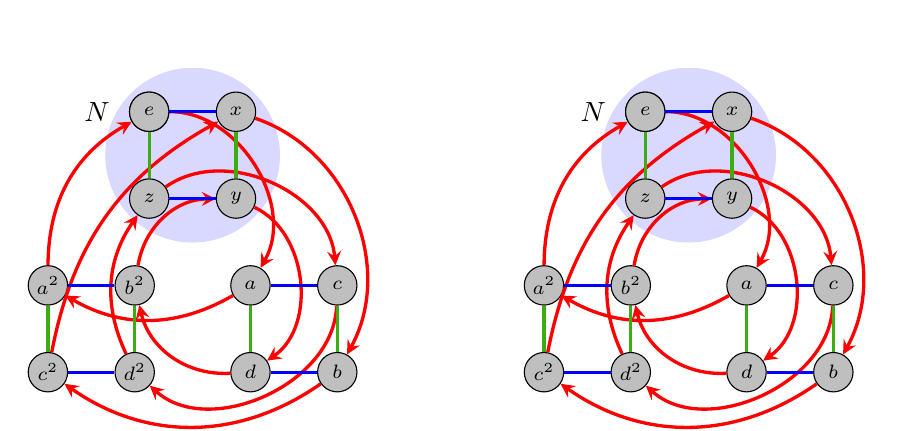
\begin{tikzpicture}[scale=1.05]
        \tikzstyle{v} = [circle, draw, fill=lightgray,inner sep=0pt,
        minimum size=5mm]
        \tikzstyle{every node}=[font=\scriptsize]
        %% N version
        \begin{scope}[shift={(0,-1.1)},scale=.7] 
            \draw[cosetBlue, fill=cosetBlue] (2.5,3.75) circle (15mm);
            \node (e) at (1.75,4.5) [v] {$e$};
            \node (x) at (3.25,4.5) [v] {$x$};
            \node (z) at (1.75,3) [v] {$z$};
            \node (y) at (3.25,3) [v] {$y$};
            \node (a) at (3.5,1.5) [v] {$a$};
            \node (c) at (5,1.5) [v] {$c$};
            \node (d) at (3.5,0) [v] {$d$};
            \node (b) at (5,0) [v] {$b$};
            \node (dd) at (1.5,0) [v] {$d^2$};
            \node (bb) at (1.5,1.5) [v] {$b^2$};
            \node (aa) at (0,1.5) [v] {$a^2$};
            \node (cc) at (0,0) [v] {$c^2$};
            \draw [r] (x) to [bend left=50] (b);
            \draw [r] (e) to [bend left=60] (a);
            \draw [r] (z) to [bend left=60] (c);
            \draw [r] (y) to [bend left=60] (d);
            \draw [r] (a) to [bend left] (aa);
            \draw [r] (b) to [bend left=35] (cc);
            \draw [r] (c) to [bend left=65] (dd);
            \draw [r] (d) to [bend left=40] (bb);
            \draw [r] (aa) to [bend left] (e);
            \draw [r] (bb) to [bend left=40] (y);
            \draw [r] (cc) to [bend left=25] (x);
            \draw [r] (dd) to [bend left] (z);
            \node at (1.75,4.5) [v] {$e$};
            \node at (.85,4.5) {\normalsize$N$};
            \draw [bb] (e) to (x);
            \draw [bb] (z) to (y);
            \draw [gg] (e) to (z);
            \draw [gg] (x) to (y);
            \draw [bb] (a) to (c);
            \draw [bb] (d) to (b);
            \draw [gg] (a) to (d);
            \draw [gg] (c) to (b);
            \draw [bb] (aa) to (bb);
            \draw [bb] (cc) to (dd);
            \draw [gg] (aa) to (cc);
            \draw [gg] (bb) to (dd);
        \end{scope}
        \begin{scope}[shift={(6,-1.1)},scale=.7] 
            \draw[cosetBlue, fill=cosetBlue] (2.5,3.75) circle (15mm);
            \node (e) at (1.75,4.5) [v] {$e$};
            \node (x) at (3.25,4.5) [v] {$x$};
            \node (z) at (1.75,3) [v] {$z$};
            \node (y) at (3.25,3) [v] {$y$};
            \node (a) at (3.5,1.5) [v] {$a$};
            \node (c) at (5,1.5) [v] {$c$};
            \node (d) at (3.5,0) [v] {$d$};
            \node (b) at (5,0) [v] {$b$};
            \node (dd) at (1.5,0) [v] {$d^2$};
            \node (bb) at (1.5,1.5) [v] {$b^2$};
            \node (aa) at (0,1.5) [v] {$a^2$};
            \node (cc) at (0,0) [v] {$c^2$};
            \draw [r] (x) to [bend left=50] (b);
            \draw [r] (e) to [bend left=60] (a);
            \draw [r] (z) to [bend left=60] (c);
            \draw [r] (y) to [bend left=60] (d);
            \draw [r] (a) to [bend left] (aa);
            \draw [r] (b) to [bend left=35] (cc);
            \draw [r] (c) to [bend left=65] (dd);
            \draw [r] (d) to [bend left=40] (bb);
            \draw [r] (aa) to [bend left] (e);
            \draw [r] (bb) to [bend left=40] (y);
            \draw [r] (cc) to [bend left=25] (x);
            \draw [r] (dd) to [bend left] (z);
            \node at (1.75,4.5) [v] {$e$};
            \node at (.85,4.5) {\normalsize$N$};
            \draw [bb] (e) to (x);
            \draw [bb] (z) to (y);
            \draw [gg] (e) to (z);
            \draw [gg] (x) to (y);
            \draw [bb] (a) to (c);
            \draw [bb] (d) to (b);
            \draw [gg] (a) to (d);
            \draw [gg] (c) to (b);
            \draw [bb] (aa) to (bb);
            \draw [bb] (cc) to (dd);
            \draw [gg] (aa) to (cc);
            \draw [gg] (bb) to (dd);
        \end{scope}
    \end{tikzpicture}
\]

Ran outta room, see next page
\pagebreak

For part (d), subgroup $K$ (why am I giving you 5 copies?):

\[
    \hspace*{-3mm}
    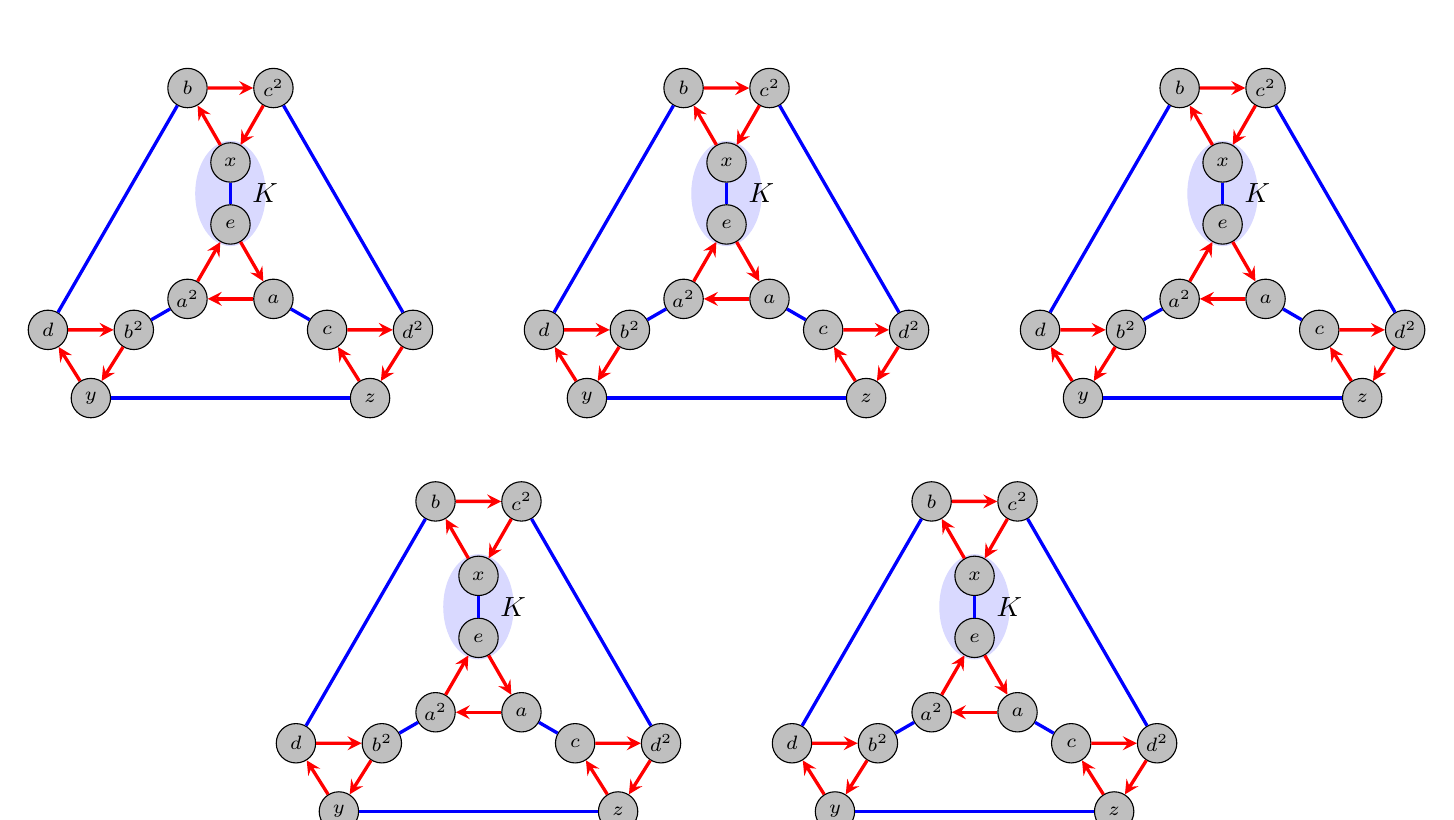
\begin{tikzpicture}[scale=1.05]
        \tikzstyle{v} = [circle, draw, fill=lightgray,inner sep=0pt,
        minimum size=5mm]
        \tikzstyle{every node}=[font=\scriptsize]
        %% K version
        \begin{scope}[shift={(0,0)},scale=.6]
            \draw[cosetBlue, fill=cosetBlue] (0,1.625) ellipse (.7 and 1.05);
            \node (l1) at (0,2.25) [v] {$x$};
            \node (l2) at (-.866,3.75) [v] {$b$};
            \node (t1) at (0,1) [v] {$e$};
            \node (t2) at (-.866,-.5) [v] {$a^2$};
            \node (t3) at (.866,-.5) [v] {$a$};
            \node (l3) at (.866,3.75) [v] {$c^2$};
            \node (r1) at (3.68,-1.125) [v] {$d^2$};
            \node (r2) at (2.814,-2.5) [v] {$z$};
            \node (r3) at (1.948,-1.125) [v] {$c$};
            \node (m2) at (-1.948,-1.125) [v] {$b^2$};
            \node (m1) at (-3.68,-1.125) [v] {$d$};
            \node (m3) at (-2.814,-2.5) [v] {$y$};
            \node at (.7,1.625) {\normalsize$K$};
            \draw [bb] (l2) to (m1);
            \draw [bb] (m2) to (t2);
            \draw [bb] (r2) to (m3);
            \draw [bb] (l1) to (t1);
            \draw [bb] (l3) to (r1);
            \draw [bb] (r3) to (t3);
            \draw [r] (l1) to (l2);
            \draw [r] (l2) to (l3);
            \draw [r] (l3) to (l1);
            \draw [r] (t1) to (t3);
            \draw [r] (t2) to (t1);
            \draw [r] (t3) to (t2);
            \draw [r] (r1) to (r2);
            \draw [r] (r2) to (r3);
            \draw [r] (r3) to (r1);
            \draw [r] (m1) to (m2);
            \draw [r] (m2) to (m3);
            \draw [r] (m3) to (m1);
        \end{scope}
        \begin{scope}[shift={(6,0)},scale=.6]
            \draw[cosetBlue, fill=cosetBlue] (0,1.625) ellipse (.7 and 1.05);
            \node (l1) at (0,2.25) [v] {$x$};
            \node (l2) at (-.866,3.75) [v] {$b$};
            \node (t1) at (0,1) [v] {$e$};
            \node (t2) at (-.866,-.5) [v] {$a^2$};
            \node (t3) at (.866,-.5) [v] {$a$};
            \node (l3) at (.866,3.75) [v] {$c^2$};
            \node (r1) at (3.68,-1.125) [v] {$d^2$};
            \node (r2) at (2.814,-2.5) [v] {$z$};
            \node (r3) at (1.948,-1.125) [v] {$c$};
            \node (m2) at (-1.948,-1.125) [v] {$b^2$};
            \node (m1) at (-3.68,-1.125) [v] {$d$};
            \node (m3) at (-2.814,-2.5) [v] {$y$};
            \node at (.7,1.625) {\normalsize$K$};
            \draw [bb] (l2) to (m1);
            \draw [bb] (m2) to (t2);
            \draw [bb] (r2) to (m3);
            \draw [bb] (l1) to (t1);
            \draw [bb] (l3) to (r1);
            \draw [bb] (r3) to (t3);
            \draw [r] (l1) to (l2);
            \draw [r] (l2) to (l3);
            \draw [r] (l3) to (l1);
            \draw [r] (t1) to (t3);
            \draw [r] (t2) to (t1);
            \draw [r] (t3) to (t2);
            \draw [r] (r1) to (r2);
            \draw [r] (r2) to (r3);
            \draw [r] (r3) to (r1);
            \draw [r] (m1) to (m2);
            \draw [r] (m2) to (m3);
            \draw [r] (m3) to (m1);
        \end{scope}
        \begin{scope}[shift={(12,0)},scale=.6]
            \draw[cosetBlue, fill=cosetBlue] (0,1.625) ellipse (.7 and 1.05);
            \node (l1) at (0,2.25) [v] {$x$};
            \node (l2) at (-.866,3.75) [v] {$b$};
            \node (t1) at (0,1) [v] {$e$};
            \node (t2) at (-.866,-.5) [v] {$a^2$};
            \node (t3) at (.866,-.5) [v] {$a$};
            \node (l3) at (.866,3.75) [v] {$c^2$};
            \node (r1) at (3.68,-1.125) [v] {$d^2$};
            \node (r2) at (2.814,-2.5) [v] {$z$};
            \node (r3) at (1.948,-1.125) [v] {$c$};
            \node (m2) at (-1.948,-1.125) [v] {$b^2$};
            \node (m1) at (-3.68,-1.125) [v] {$d$};
            \node (m3) at (-2.814,-2.5) [v] {$y$};
            \node at (.7,1.625) {\normalsize$K$};
            \draw [bb] (l2) to (m1);
            \draw [bb] (m2) to (t2);
            \draw [bb] (r2) to (m3);
            \draw [bb] (l1) to (t1);
            \draw [bb] (l3) to (r1);
            \draw [bb] (r3) to (t3);
            \draw [r] (l1) to (l2);
            \draw [r] (l2) to (l3);
            \draw [r] (l3) to (l1);
            \draw [r] (t1) to (t3);
            \draw [r] (t2) to (t1);
            \draw [r] (t3) to (t2);
            \draw [r] (r1) to (r2);
            \draw [r] (r2) to (r3);
            \draw [r] (r3) to (r1);
            \draw [r] (m1) to (m2);
            \draw [r] (m2) to (m3);
            \draw [r] (m3) to (m1);
        \end{scope}
        \begin{scope}[shift={(3,-5)},scale=.6]
            \draw[cosetBlue, fill=cosetBlue] (0,1.625) ellipse (.7 and 1.05);
            \node (l1) at (0,2.25) [v] {$x$};
            \node (l2) at (-.866,3.75) [v] {$b$};
            \node (t1) at (0,1) [v] {$e$};
            \node (t2) at (-.866,-.5) [v] {$a^2$};
            \node (t3) at (.866,-.5) [v] {$a$};
            \node (l3) at (.866,3.75) [v] {$c^2$};
            \node (r1) at (3.68,-1.125) [v] {$d^2$};
            \node (r2) at (2.814,-2.5) [v] {$z$};
            \node (r3) at (1.948,-1.125) [v] {$c$};
            \node (m2) at (-1.948,-1.125) [v] {$b^2$};
            \node (m1) at (-3.68,-1.125) [v] {$d$};
            \node (m3) at (-2.814,-2.5) [v] {$y$};
            \node at (.7,1.625) {\normalsize$K$};
            \draw [bb] (l2) to (m1);
            \draw [bb] (m2) to (t2);
            \draw [bb] (r2) to (m3);
            \draw [bb] (l1) to (t1);
            \draw [bb] (l3) to (r1);
            \draw [bb] (r3) to (t3);
            \draw [r] (l1) to (l2);
            \draw [r] (l2) to (l3);
            \draw [r] (l3) to (l1);
            \draw [r] (t1) to (t3);
            \draw [r] (t2) to (t1);
            \draw [r] (t3) to (t2);
            \draw [r] (r1) to (r2);
            \draw [r] (r2) to (r3);
            \draw [r] (r3) to (r1);
            \draw [r] (m1) to (m2);
            \draw [r] (m2) to (m3);
            \draw [r] (m3) to (m1);
        \end{scope}
        \begin{scope}[shift={(9,-5)},scale=.6]
            \draw[cosetBlue, fill=cosetBlue] (0,1.625) ellipse (.7 and 1.05);
            \node (l1) at (0,2.25) [v] {$x$};
            \node (l2) at (-.866,3.75) [v] {$b$};
            \node (t1) at (0,1) [v] {$e$};
            \node (t2) at (-.866,-.5) [v] {$a^2$};
            \node (t3) at (.866,-.5) [v] {$a$};
            \node (l3) at (.866,3.75) [v] {$c^2$};
            \node (r1) at (3.68,-1.125) [v] {$d^2$};
            \node (r2) at (2.814,-2.5) [v] {$z$};
            \node (r3) at (1.948,-1.125) [v] {$c$};
            \node (m2) at (-1.948,-1.125) [v] {$b^2$};
            \node (m1) at (-3.68,-1.125) [v] {$d$};
            \node (m3) at (-2.814,-2.5) [v] {$y$};
            \node at (.7,1.625) {\normalsize$K$};
            \draw [bb] (l2) to (m1);
            \draw [bb] (m2) to (t2);
            \draw [bb] (r2) to (m3);
            \draw [bb] (l1) to (t1);
            \draw [bb] (l3) to (r1);
            \draw [bb] (r3) to (t3);
            \draw [r] (l1) to (l2);
            \draw [r] (l2) to (l3);
            \draw [r] (l3) to (l1);
            \draw [r] (t1) to (t3);
            \draw [r] (t2) to (t1);
            \draw [r] (t3) to (t2);
            \draw [r] (r1) to (r2);
            \draw [r] (r2) to (r3);
            \draw [r] (r3) to (r1);
            \draw [r] (m1) to (m2);
            \draw [r] (m2) to (m3);
            \draw [r] (m3) to (m1);
        \end{scope}
    \end{tikzpicture}
\]

Now with $H$ highlighted instead of $K$

\[
    \hspace*{-3mm}
    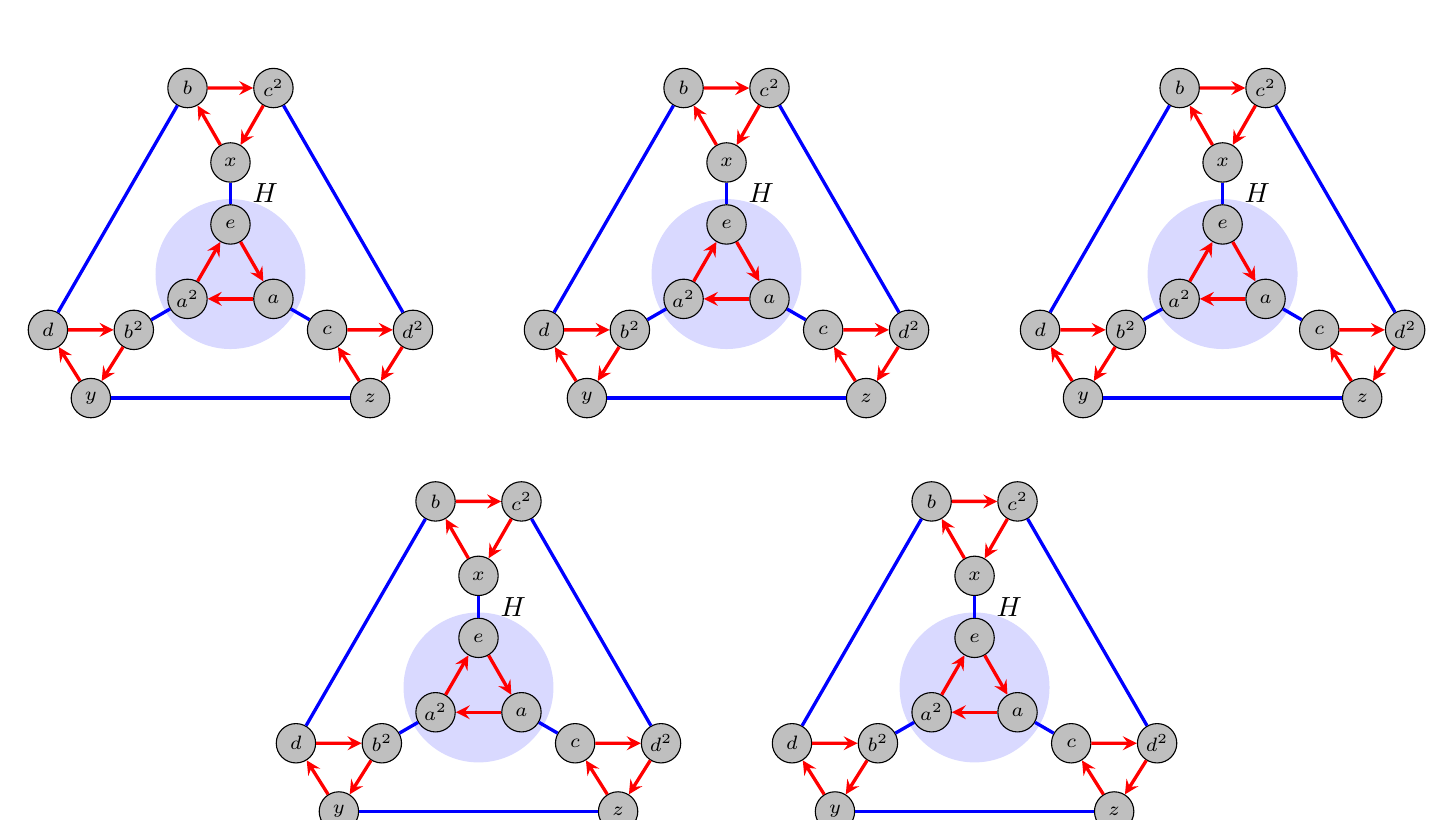
\begin{tikzpicture}[scale=1.05]
        \tikzstyle{v} = [circle, draw, fill=lightgray,inner sep=0pt,
        minimum size=5mm]
        \tikzstyle{every node}=[font=\scriptsize]
        %% K version
        \begin{scope}[shift={(0,0)},scale=.6]
            \draw[cosetBlue, fill=cosetBlue] (0,0) ellipse (1.5 and 1.5);
            \node (l1) at (0,2.25) [v] {$x$};
            \node (l2) at (-.866,3.75) [v] {$b$};
            \node (t1) at (0,1) [v] {$e$};
            \node (t2) at (-.866,-.5) [v] {$a^2$};
            \node (t3) at (.866,-.5) [v] {$a$};
            \node (l3) at (.866,3.75) [v] {$c^2$};
            \node (r1) at (3.68,-1.125) [v] {$d^2$};
            \node (r2) at (2.814,-2.5) [v] {$z$};
            \node (r3) at (1.948,-1.125) [v] {$c$};
            \node (m2) at (-1.948,-1.125) [v] {$b^2$};
            \node (m1) at (-3.68,-1.125) [v] {$d$};
            \node (m3) at (-2.814,-2.5) [v] {$y$};
            \node at (.7,1.625) {\normalsize$H$};
            \draw [bb] (l2) to (m1);
            \draw [bb] (m2) to (t2);
            \draw [bb] (r2) to (m3);
            \draw [bb] (l1) to (t1);
            \draw [bb] (l3) to (r1);
            \draw [bb] (r3) to (t3);
            \draw [r] (l1) to (l2);
            \draw [r] (l2) to (l3);
            \draw [r] (l3) to (l1);
            \draw [r] (t1) to (t3);
            \draw [r] (t2) to (t1);
            \draw [r] (t3) to (t2);
            \draw [r] (r1) to (r2);
            \draw [r] (r2) to (r3);
            \draw [r] (r3) to (r1);
            \draw [r] (m1) to (m2);
            \draw [r] (m2) to (m3);
            \draw [r] (m3) to (m1);
        \end{scope}
        \begin{scope}[shift={(6,0)},scale=.6]
            \draw[cosetBlue, fill=cosetBlue] (0,0) ellipse (1.5 and 1.5);
            \node (l1) at (0,2.25) [v] {$x$};
            \node (l2) at (-.866,3.75) [v] {$b$};
            \node (t1) at (0,1) [v] {$e$};
            \node (t2) at (-.866,-.5) [v] {$a^2$};
            \node (t3) at (.866,-.5) [v] {$a$};
            \node (l3) at (.866,3.75) [v] {$c^2$};
            \node (r1) at (3.68,-1.125) [v] {$d^2$};
            \node (r2) at (2.814,-2.5) [v] {$z$};
            \node (r3) at (1.948,-1.125) [v] {$c$};
            \node (m2) at (-1.948,-1.125) [v] {$b^2$};
            \node (m1) at (-3.68,-1.125) [v] {$d$};
            \node (m3) at (-2.814,-2.5) [v] {$y$};
            \node at (.7,1.625) {\normalsize$H$};
            \draw [bb] (l2) to (m1);
            \draw [bb] (m2) to (t2);
            \draw [bb] (r2) to (m3);
            \draw [bb] (l1) to (t1);
            \draw [bb] (l3) to (r1);
            \draw [bb] (r3) to (t3);
            \draw [r] (l1) to (l2);
            \draw [r] (l2) to (l3);
            \draw [r] (l3) to (l1);
            \draw [r] (t1) to (t3);
            \draw [r] (t2) to (t1);
            \draw [r] (t3) to (t2);
            \draw [r] (r1) to (r2);
            \draw [r] (r2) to (r3);
            \draw [r] (r3) to (r1);
            \draw [r] (m1) to (m2);
            \draw [r] (m2) to (m3);
            \draw [r] (m3) to (m1);
        \end{scope}
        \begin{scope}[shift={(12,0)},scale=.6]
            \draw[cosetBlue, fill=cosetBlue] (0,0) ellipse (1.5 and 1.5);
            \node (l1) at (0,2.25) [v] {$x$};
            \node (l2) at (-.866,3.75) [v] {$b$};
            \node (t1) at (0,1) [v] {$e$};
            \node (t2) at (-.866,-.5) [v] {$a^2$};
            \node (t3) at (.866,-.5) [v] {$a$};
            \node (l3) at (.866,3.75) [v] {$c^2$};
            \node (r1) at (3.68,-1.125) [v] {$d^2$};
            \node (r2) at (2.814,-2.5) [v] {$z$};
            \node (r3) at (1.948,-1.125) [v] {$c$};
            \node (m2) at (-1.948,-1.125) [v] {$b^2$};
            \node (m1) at (-3.68,-1.125) [v] {$d$};
            \node (m3) at (-2.814,-2.5) [v] {$y$};
            \node at (.7,1.625) {\normalsize$H$};
            \draw [bb] (l2) to (m1);
            \draw [bb] (m2) to (t2);
            \draw [bb] (r2) to (m3);
            \draw [bb] (l1) to (t1);
            \draw [bb] (l3) to (r1);
            \draw [bb] (r3) to (t3);
            \draw [r] (l1) to (l2);
            \draw [r] (l2) to (l3);
            \draw [r] (l3) to (l1);
            \draw [r] (t1) to (t3);
            \draw [r] (t2) to (t1);
            \draw [r] (t3) to (t2);
            \draw [r] (r1) to (r2);
            \draw [r] (r2) to (r3);
            \draw [r] (r3) to (r1);
            \draw [r] (m1) to (m2);
            \draw [r] (m2) to (m3);
            \draw [r] (m3) to (m1);
        \end{scope}
        \begin{scope}[shift={(3,-5)},scale=.6]
            \draw[cosetBlue, fill=cosetBlue] (0,0) ellipse (1.5 and 1.5);
            \node (l1) at (0,2.25) [v] {$x$};
            \node (l2) at (-.866,3.75) [v] {$b$};
            \node (t1) at (0,1) [v] {$e$};
            \node (t2) at (-.866,-.5) [v] {$a^2$};
            \node (t3) at (.866,-.5) [v] {$a$};
            \node (l3) at (.866,3.75) [v] {$c^2$};
            \node (r1) at (3.68,-1.125) [v] {$d^2$};
            \node (r2) at (2.814,-2.5) [v] {$z$};
            \node (r3) at (1.948,-1.125) [v] {$c$};
            \node (m2) at (-1.948,-1.125) [v] {$b^2$};
            \node (m1) at (-3.68,-1.125) [v] {$d$};
            \node (m3) at (-2.814,-2.5) [v] {$y$};
            \node at (.7,1.625) {\normalsize$H$};
            \draw [bb] (l2) to (m1);
            \draw [bb] (m2) to (t2);
            \draw [bb] (r2) to (m3);
            \draw [bb] (l1) to (t1);
            \draw [bb] (l3) to (r1);
            \draw [bb] (r3) to (t3);
            \draw [r] (l1) to (l2);
            \draw [r] (l2) to (l3);
            \draw [r] (l3) to (l1);
            \draw [r] (t1) to (t3);
            \draw [r] (t2) to (t1);
            \draw [r] (t3) to (t2);
            \draw [r] (r1) to (r2);
            \draw [r] (r2) to (r3);
            \draw [r] (r3) to (r1);
            \draw [r] (m1) to (m2);
            \draw [r] (m2) to (m3);
            \draw [r] (m3) to (m1);
        \end{scope}
        \begin{scope}[shift={(9,-5)},scale=.6]
            \draw[cosetBlue, fill=cosetBlue] (0,0) ellipse (1.5 and 1.5);
            \node (l1) at (0,2.25) [v] {$x$};
            \node (l2) at (-.866,3.75) [v] {$b$};
            \node (t1) at (0,1) [v] {$e$};
            \node (t2) at (-.866,-.5) [v] {$a^2$};
            \node (t3) at (.866,-.5) [v] {$a$};
            \node (l3) at (.866,3.75) [v] {$c^2$};
            \node (r1) at (3.68,-1.125) [v] {$d^2$};
            \node (r2) at (2.814,-2.5) [v] {$z$};
            \node (r3) at (1.948,-1.125) [v] {$c$};
            \node (m2) at (-1.948,-1.125) [v] {$b^2$};
            \node (m1) at (-3.68,-1.125) [v] {$d$};
            \node (m3) at (-2.814,-2.5) [v] {$y$};
            \node at (.7,1.625) {\normalsize$H$};
            \draw [bb] (l2) to (m1);
            \draw [bb] (m2) to (t2);
            \draw [bb] (r2) to (m3);
            \draw [bb] (l1) to (t1);
            \draw [bb] (l3) to (r1);
            \draw [bb] (r3) to (t3);
            \draw [r] (l1) to (l2);
            \draw [r] (l2) to (l3);
            \draw [r] (l3) to (l1);
            \draw [r] (t1) to (t3);
            \draw [r] (t2) to (t1);
            \draw [r] (t3) to (t2);
            \draw [r] (r1) to (r2);
            \draw [r] (r2) to (r3);
            \draw [r] (r3) to (r1);
            \draw [r] (m1) to (m2);
            \draw [r] (m2) to (m3);
            \draw [r] (m3) to (m1);
        \end{scope}
    \end{tikzpicture}
\]

\end{document}

